\documentclass[12pt,a4paper]{article}
\usepackage{times}
%\usepackage[T1]{fontenc}
%\usepackage[latin1]{inputenc}
\usepackage{amsmath}
\usepackage{amsfonts}
\usepackage{amssymb}
%\usepackage[french]{babel}
\usepackage{graphicx}
\usepackage{url}
\usepackage{dirtree}
\usepackage{xcolor}
\DeclareTextSymbol{\degre}{OT1}{23}
\usepackage{import}
\usepackage{hyperref}
\hypersetup{
    colorlinks=true,
    linkcolor=black,
    filecolor=magenta,      
    urlcolor=blue,
}

%\usepackage[a4paper]{geometry}
\usepackage{pdfpages}

\urlstyle{same}

\begin{document}
\newcommand{\fig}[1]{Fig.#1}
\begin{titlepage}
\begin{center}

\textsc{\huge{SPASSO:Software Package for an Adaptive Satellite-based Sampling for Oceanographic cruises}}\\
\vspace{1\baselineskip}
\textsc{\LARGE{User Guide}}\\
\vspace{1\baselineskip}
\textit{{\large{A. Ricout, A.M. Doglioli, S. Barrillon, A. Della Penna, A. Petrenko, L. Rousselet F. Nencioli, A. De Verneil, C.Yohia, F. d'Ovidio,}}}\\ %Frederic Briol
\vspace{1\baselineskip}
\textsc{\large{Mediterranean Institute of Oceanography (M.I.O.)}}\\
\textsc{\normalsize{Campus de Luminy, 13288 MARSEILLE cedex 9, France}}\\
\begin{figure}[h!]
\centerline{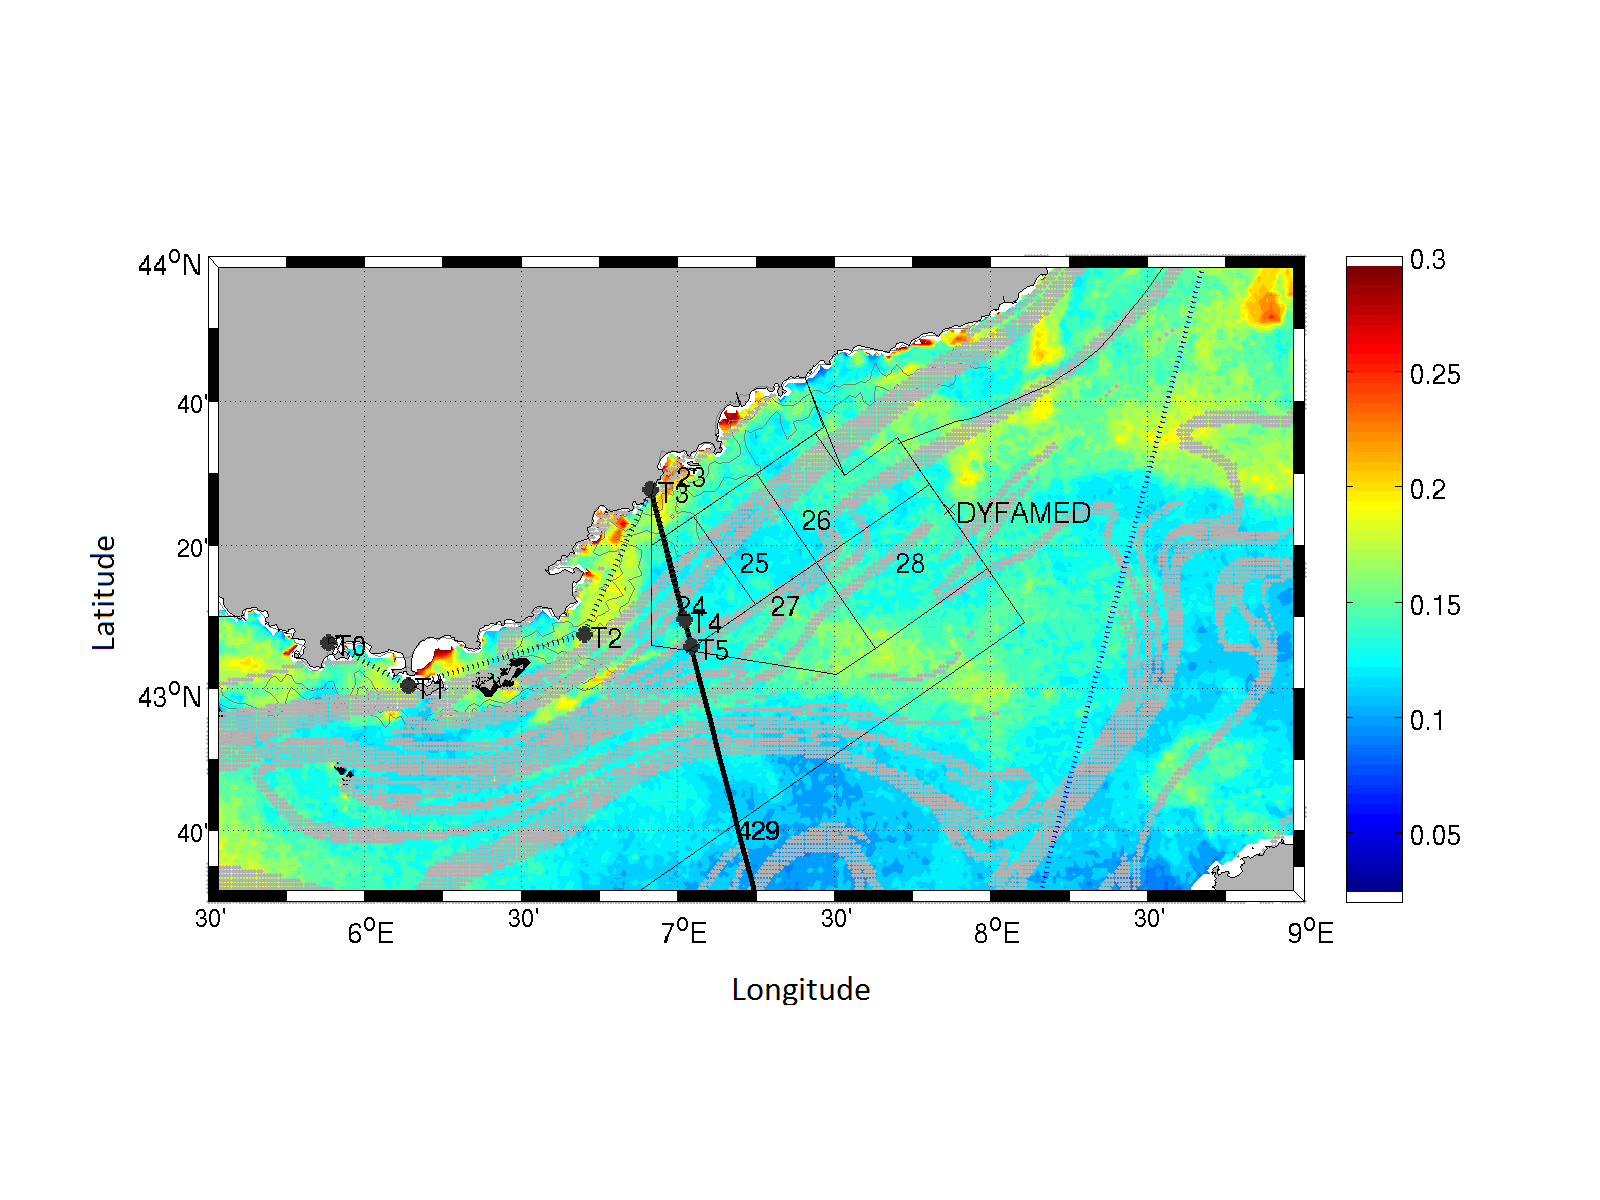
\includegraphics[scale=0.41]{Figures/20151023_d-OC_CNR-L3-CHL-MedOC3AD4_A_1KM-MED-NRT.png}}
%\caption{}
\end{figure}
\vfill
\today{ v1.}
\end{center}
%\end{sffamily}
\end{titlepage}
\makeatother


% \section{Introduction}
{\textbf{\fontsize{19}{40}\selectfont Introduction}} \\
\\
%\textcolor{blue}{TO BE DONE} \\
\\
The horizontal mesoscale and submesoscale circulation variability strongly affects biogeochemical budgets. Therefor it's a real challenge during in situ measurements to follow a sampling strategy that will provide a specific representative situation. 
That's why d'Ovidio et al. (2012) developped several diagnostics based on the study of near-real time altimetry data which allow almost instantly to map physical structures of biogeochemical interest (fronts, eddy core, temperature filaments). At high resolution this analysis permits to identify in advance potential biogeochemical regions to sample or even where phytoplanktonic bloom might occur. This strategy has already been tested during many campaigns such as Latex10 (2010), KEOPS2 (2011) or even STRASSE (2012) to identify the center of an eddy as the most stable region.\\
Based on these previous works \href{https://spasso.mio.osupytheas.fr/}{SPASSO} \footnote{https://spasso.mio.osupytheas.fr}\textbf{•} has been updated in order to make it available for any oceanographic campaign, such as the OUTPACE cruise that has used this new sampling strategy in February and March 2015 or also the FUMSECK cruise in May 2019. To make the package more comprehensive processing maps of ocean color data (Chlorophylle -a concentration) and Sea Surface Temperature (SST) was added to the lagrangian analysis that uses u and v components of velocity derived from Sea Surface Height. The altimeter products, for SSH and u,v components, are produced by Ssalto/Duacs and distributed by CMEMS with support of CNES \footnote{https://www.cnes.fr}. The SPASSO software is in charge of collecting online data, treating them to make maps of the different parameters (Chlorophylle -a presence, SST and Chl-a, near-real time velocity maps, diagnostics for lagrangian analysis) and publish them on the web \footnote{https://spasso.mio.osupytheas.fr/FUMSECK/FIGURES} so that they will be available directly from the vessel. \\
This following guide take as DEMO cruise example the last FUMSECK cruise done in May 2019 in the golf of Genoa with its related satellite products. You can adapt the DEMO cruise to your own objectives of oceanographic cruise.
\newpage
\tableofcontents
\newpage

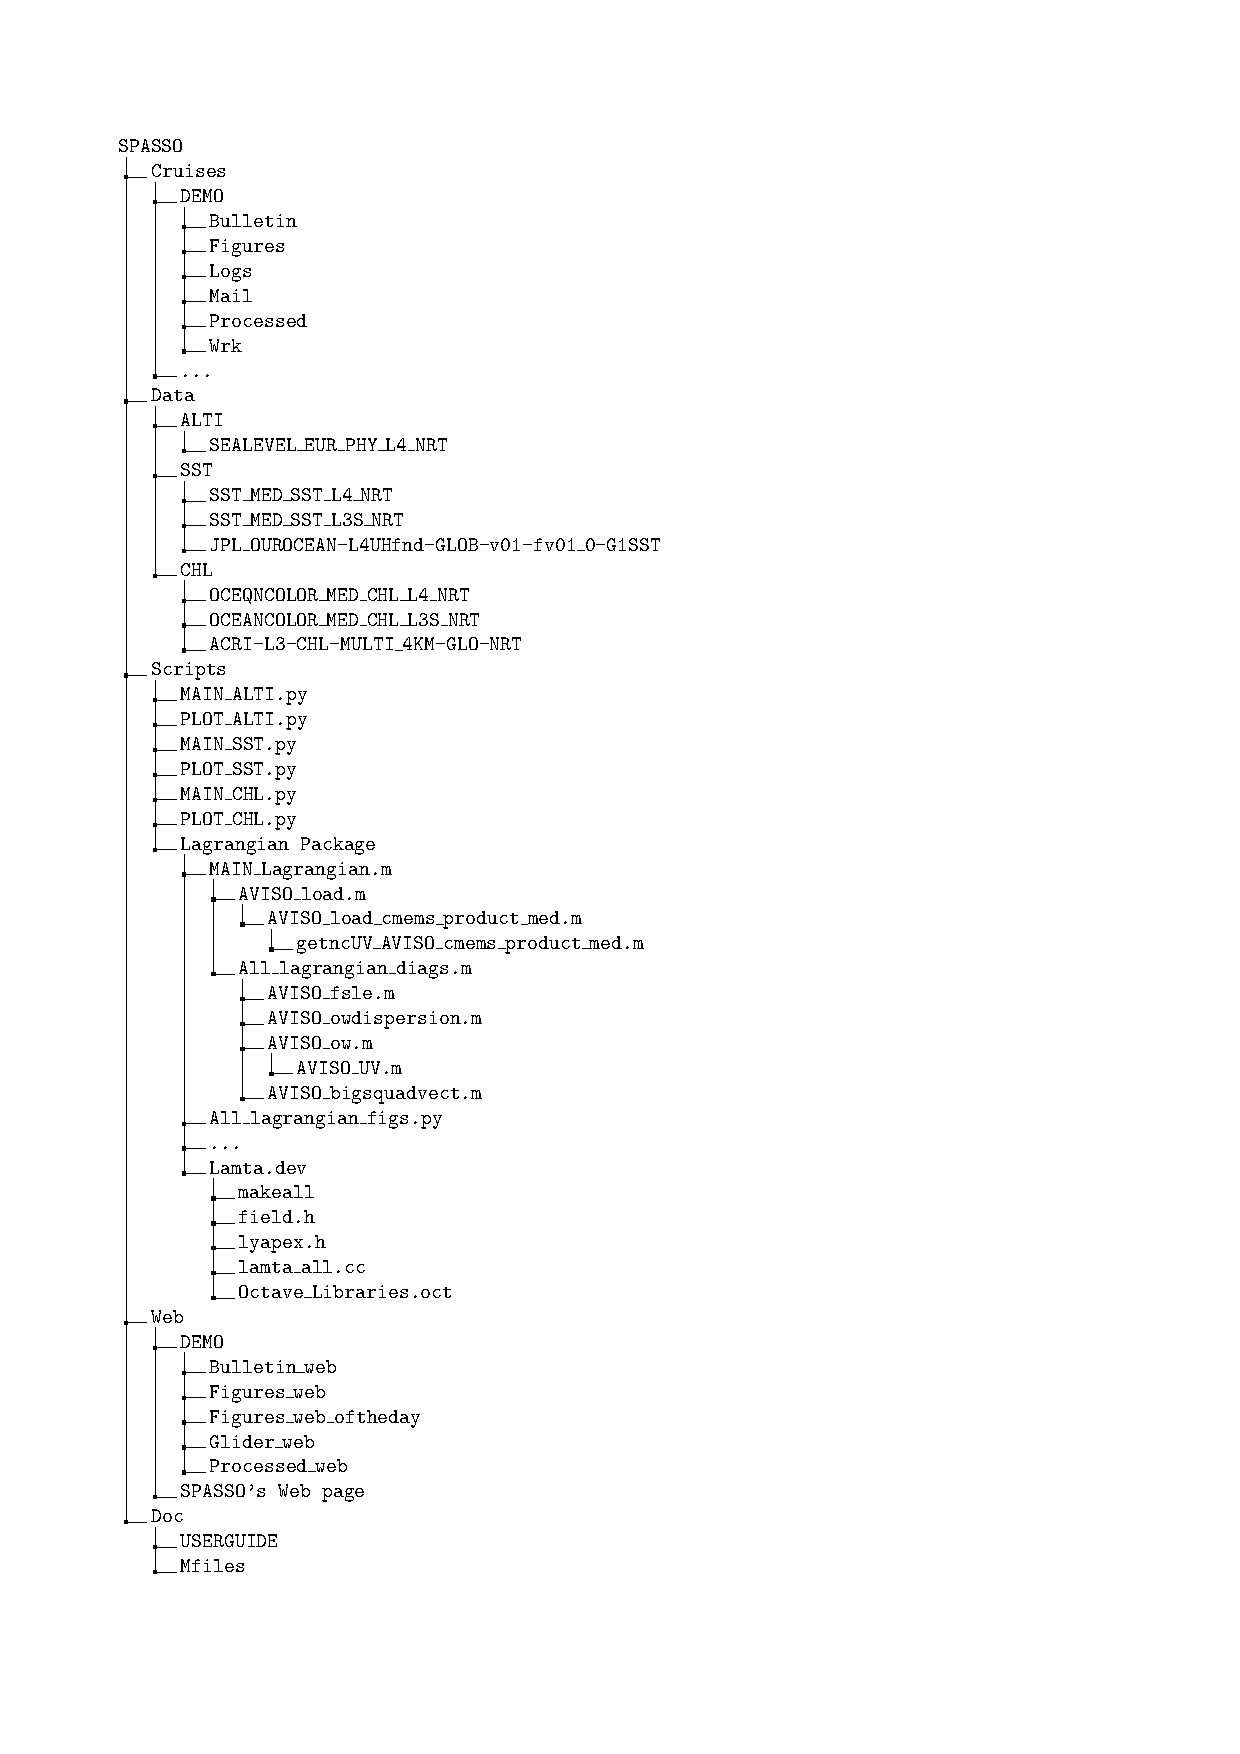
\includepdf[scale=0.75, pagecommand=\section{Files directory and contents}]{diagram_tree.pdf}
The software package is organized from the previou directory tree. Here is a quick description of the content of those files: \\
\\
\noindent \texttt{-Cruises/}: previous or in progress cruise directories \newline
\indent \texttt{-DEMO/}: \newline
\indent \indent \texttt{-Bulletin/}: daily bulletin reporting oceanographic conditions \newline
\indent \indent \texttt{-Figures/}: all .png figures processed on a daily basis by python scripts \newline
\indent \indent \texttt{-Logs/}: Event history .txt file that records linux comments during \textit{spasso.sh} processing \newline
\indent \indent \texttt{-Mail/}:  \newline
\indent \indent \texttt{-Processed/}: all .mat data processed by Python and Octave scripts and compressed during \textit{spasso.sh} processing \newline
\indent \indent \texttt{-Wrk/}: file where netcdf files are duplicated from Data/: and processed by Python and Octave scripts \newline
\noindent \texttt{-Data/}: near-real-time data in NetCDF files format downloaded during \textit{spasso.sh} processing \newline
\indent \texttt{-ALTI/}: near-real-time sea surface height and UV components CMEMS netcdf files \newline 
\indent \texttt{-SST/}:  near-real-time sea surface temmperature CMEMS and JPL netcdf files \newline
\indent \texttt{-CHL/}: near-real-time chlorophylle -a CMEMS netcdf files \newline
\texttt{-Scripts/}: python and octave scripts to plot satellite data \newline
\indent Lagrangian\_package: python and octave scripts to make Lagrangian analysis \newline
\indent \indent lamta.dev: C scripts used in Lagrangian analysis \newline
\noindent \texttt{-Web/}: file where bulletins, figures and data could be recorded and synchronized online on your own web page (to do it, you have to generate an index\_web\_page.html).\newline

\section{Data}
All the products detailed hereafter are provided in NetCDF files format, are treated daily and analysed in near-real time, over a chosen area (follows below the example for a Mediterranean geographical coverage 90\degre N,180\degre E ; 90\degre S,180\degre W).
\subsection{Altimetric Data}
The altimetric product SEALEVEL\_EUR\_PHY\_L4\_NRT\_OBSERVATIONS\_008 \\ \_060 is processed by the DUACS multi-mission altimeter data processing system, merging the different altimeter measurements available (at one given time, to make sure to have the best data quality). \newline 
This dataset: dataset-duacs-nrt-europe-merged-allsat-phy-l4 is gridded on a 0.125\degre x 0.125\degre resolution Cartesian grid and contains different variables: \newline
- Sea Suface Height (SSH), above reference ellispoid (m) \newline
- U/V Surface Geostrophic Eastward/Northward Sea Water Velocity, with absolute and anomalie values (m/s) \newline 
Note that the DUAC dataset is available via the CMEMS website  (with 
registration): \url{http://marine.copernicus.eu/services-portfolio/access-to-products/?option=com_csw&view=details& \\ product_id=SEALEVEL\_EUR\_PHY\_L4\_NRT\_OBSERVATIONS\_008\_060} 

%%%%%%% SEALEVEL_MED %%%%%%%%%
%The altimetric product SEALEVEL\_MED\_PHY\_L4\_NRT\_OBSERVATIONS\_008 \\ \_050 is processed by the DUACS multimission altimeter data processing system, merging of the different altimeter measurements available (at one given time, to make sure to have the best data quality). \newline 
%This dataset: dataset-duacs-nrt-med-merged-allsat-phy-l4 is gridded on a 0.125\degre x 0.125\degre resolution Cartesian grid and contains different variables: \newline
%- Sea Suface Height (SSH), above geoide and sea level (m) \newline
%- U/V Surface Geostrophic Northward/Eastward Sea Water Velocity, with absolute and anomalie values (m/s) \newline 
%Note that the DUAC dataset is available via the CMEMS website  (with 
%registration): \url{http://marine.copernicus.eu/services-portfolio/access-to-products/?option=com_csw&view=details& \\ product_id=SEALEVEL\_MED\_PHY\_L4\_NRT\_OBSERVATIONS\_008\_050} 


%The Ssalto/Duacs products are gridded on a $\frac{1}{4}$ $\times$ $\frac{1}{4}\degre$ resolution Cartesian grid since April 15$^{th}$ 2014. Before this deadline AVISO NetCDF files used different variable names and formats gridded on a $\frac{1}{3}\degre$ Mercator grid. From those changes resulted an entire update of all scripts and function to make them run with both previous and new NetCDF files format. Therefor it is still possible to run the package with former AVISO files. \newline
%To provide new maps every day, AVISO near-real-time MADT (Maps of Absolute Dynamic Topography) products have been used to retrieve two types of data: \newline
%- SSH data gridded above the geoid (m) \newline
%- u and v components of velocity using geostrophic approximation (m/s)\\
%The default option is to treat 'all-sat-merged' data meaning that those data are obtained using all satellites available at one given time, to make sure to have the best data quality. \newline
 
\subsection{Ocean color Data}
The Ocean Color Data OCEANCOLOUR\_GLO\_CHL\_L3\_NRT\_OBSERVATIONS \\ \_009\_032 product providing Chlorophyll-a and Optics dataset is distributed by ACRI-ST company. It is based on the Copernicus-GlobColour processing including MODIS-Aqua and VIIRS-N satellite data. \newline 
This dataset:-oc-glo-chl-multi\_a-l3-av\_4km\_daily-rt-v02 is given on a $\frac{1}{24}$ $\times$ $\frac{1}{24}\degre$ resolution horizontal grid, about 4km, highest resolution available for this product, and provides a single variable: \newline
- mass concentration of chlorophyll-a (CHL) in the sea water (mg/m$^{3}$) \newline
Note that the ACRI-ST product is available via the CMEMS website  (with 
registration): \url{http://marine.copernicus.eu/services-portfolio/access-to-products/?option=com_csw&view=details&product_id=OCEANCOLOUR_GLO_CHL_L3_NRT_OBSERVATIONS_009_032}
\\
\\
%AR%
%-  L3 Chlorophyll concentration (CHL GSM) (mg/m$^{3}$) \newline 
%Optic data: \newline
%- Reflectance (RRS) (nm) (sr$^{-1}$) \newline
%- Transparency (ZSD) (nm) (m$^{-1}$) \newline
%- Suspended Matter (SPM) (g/m$^{3}$) \newline 
%- Particulate Backscattering (BBP) (nm) (m$^{-1}$) \newline
%- Secchi Transparency (ZSD) (m) \newline
%- Diffuse Attenuation (KD490) (nm) (m$^{-1}$) \newline
%- Absorption Coefficient (ADG/CDM) (nm) (m$^{-1}$) \\
%AR%
The Ocean Color Data OCEANCOLOUR\_MED\_CHL\_L3\_NRT\_OBSERVATIONS \\ \_009\_040 product providing Chlorophyll-a and Optics dataset is distributed by the Global Ocean Satellite monitoring and marine ecosystem study group (GOS) of the Italian National Research Council (CNR). It is based on the Copernicus-GlobColour processing including MODIS-Aqua and VIIRS-N satellite data. \newline 
This dataset:-oc-med-chl-multi-l3-chl\_1km\_daily-rt-v02 is obtained by means of the Mediterranean Ocean Colour regional algorithms and given on a 0.125\degre x 0.125\degre  resolution horizontal grid, about 1km, highest resolution available for this product, and provides a single variable: \newline
- mass concentration of chlorophyll-a (CHL) in the sea water (mg/m$^{3}$) \newline
Note that the ACRI-ST product is available via the CMEMS website  (with 
registration): \url{http://marine.copernicus.eu/services-portfolio/access-to-products/?option=com_csw&view=details&product_id=OEANCOLOUR\_MED\_CHL\_L3\_NRT\_OBSERVATIONS\_009\_040}
\\
\\
%For Ocean Color data the default option is to use the highest resolution (4 km) to have a better representation of small scale features. Chlorophyll -a and Sea Surface Temperature are mapped using Level 3 Standard Mapped Image products which are image representations of binned data products. The oceancolor website \footnote{oceancolor.gsfc.nasa.gov} provide every day data which permits, the same way as AVISO products, to get near-real-time data.\\
%Chlorophyll -a concentration is derived from an algorithm that describes the polynomial best fit that relates the log-transformed geophysical variable to a log-transformed ratio of remote-sensing reflectances with:
%\begin{center}
%\begin{equation}
%X = log10(Rrs1 / Rrs2)
%\end{equation}
%\begin{equation}
%chlor\_a = 10^{(a_{0} + a_{1} \times X + a_{2} \times X^{2} + a_{3} \times X^{3} + a_{4} \times X^{4})}  (mg/m^{3})
%\end{equation}
%\end{center}
%where:
%\begin{itemize}
%\item Rrs1 = blue wavelength Rrs (e.g., 443, 490, or 510-nm)
%\item Rrs2 = green wavelength Rrs (e.g., 547, 555, or 565-nm)
%\end{itemize}
The Ocean Color Data OCEANCOLOUR\_MED\_CHL\_L4\_NRT\_OBSERVATIONS \\ \_009\_041 product providing Chlorophyll-a and Optics dataset is distributed by the Global Ocean Satellite monitoring and marine ecosystem study group (GOS) of the Italian National Research Council (CNR). It is based on the Copernicus-GlobColour processing including MODIS-Aqua and VIIRS-N satellite data. \newline 
This dataset:-oc-med-chl-multi-l4-chl\_1km\_daily-rt-v02 is an interpolated product based on the L3 products at 1 km resolution. These L4 daily-interpolated fields are calculated from two products: monthly-averaged and 8-day averaged. It is given in a 0.125\degre x 0.125\degre  resolution horizontal grid, about 1km, highest resolution available for this product, and provides a single variable: \newline
- mass concentration of chlorophyll-a (CHL) in the sea water (mg/m$^{3}$) \newline
Note that the ACRI-ST product is available via the CMEMS website  (with 
registration): \url{http://marine.copernicus.eu/services-portfolio/access-to-products/?option=com_csw&view=details&product_id=OEANCOLOUR\_MED\_CHL\_L4\_NRT\_OBSERVATIONS\_009\_041}
\\
\\
\subsection{Sea Surface Temperature Data} 
The Sea Surface Temperature Level 3 gridded products over the Mediterranean Sea SST\_MED\_SST\_L3S\_NRT\_OBSERVATIONS\_010\_012 is provided by the National Research Council (CNR). It is based on the merging of several satellite SST data over a 0.063\degre x 0.063\degre resolution Mediterranean sea grid. This product contains the daataset: SST\_MED\_SST\_L3S\_NRT\_OBSERVATIONS\_010\_012\_a providing a single variable: \newline 
- Sea Surface Temperature (SST) (Kelvin) \newline 
Note that the product is available via the CMEMS website  (with registration): \url{http://marine.copernicus.eu/services-portfolio/access-to-products/?option=com_csw&view=details&product_id=SST_MED_SST_L3S_NRT_OBSERVATIONS_010_012
}
\\
\\
The Sea Surface Temperature Level 4 gridded products over the Mediterranean Sea SST\_MED\_SST\_L4\_NRT\_OBSERVATIONS\_010\_004 are remotely-sensed L4 Sea Surface Temperature (SST) datasets.They are operationally produced and distributed in near-real time by the Consiglio Nazionale delle Ricerche - Gruppo di Oceanografia da Satellite (CNR-GOS). Tey are based on the merging of several satellite SST data over a 0.063\degre x 0.063\degre resolution Mediterranean sea grid. This product contains the daataset: SST\_MED\_SST\_L4\_NRT\_OBSERVATIONS\_010\_004\_a providing a single variable: \newline 
- Sea Surface Temperature (SST) (Kelvin) \newline 
Note that the product is available via the CMEMS website  (with registration): \url{http://marine.copernicus.eu/services-portfolio/access-to-products/?option=com_csw&view=details&product_id=SST_MED_SST_L4_NRT_OBSERVATIONS_010_004
}
\\ 
\\
The JPL OurOcean group provides the JPL\_OUROCEAN-L4UHfnd-GLOB-G1SST product, a Global 1km SST analysis using satellite data from multi-sensor and in situ data.This product is gridded in a 0.1\degre x 0.1\degre resolution global grid and contains the variable: \newline
- Sea Surface Temperature (SST) (Kelvin) \newline
Note that the JPL OurOcean group product is available via the NASA website  (with 
registration): \url{https://podaac.jpl.nasa.gov/datasetlist?ids=Measurement:ProcessingLevel:Variable:Availability:SpatialCoverage&values=Ocean%20Temperature:*4*:Sea%20Surface%20Temperature:NEAR_REAL_TIME:Global&view=list#}
\\
%The Sea Surface Temperature ($\degre$C) is measured using the 11 and 12 micron channels during the day but measurments are also available during the night.

\newpage

\section{Data acquisition and plot}
\subsection{Data processing}
The SPASSO package contains the shell script \textit{spasso.sh} which can be executed automatically by crontab. It downloads the NetCDF files of the day in \texttt{Data/} then makes their copy in \texttt{Wrk/}.This script executes Python and Octave scripts, contained in \texttt{/Scripts}. The structure of the Python scripts is as follows :\newline
\begin{itemize}
\item MAIN\_ALTI.py: \newline
\indent $\rightarrow$ function that extracts NetCDF variables from data files \newline
\indent $\rightarrow$ function that saves variables in .mat files in \texttt{Wrk/} \newline
\newline
\item plot\_ALTI.py: script that plots maps of SSH and velocity quiver for the studied zone, using .mat files from \texttt{Wrk/}, and saves them in .png format.\newline
\item MAIN\_CHL.py: \newline
\indent $\rightarrow$ function that extracts NetCDF variables from data files \newline
\indent $\rightarrow$ function that saves variables in .mat files in \texttt{Wrk/} \newline
\newline
\item plot\_CHL.py: script that plots maps of CHL concentration for the studied zone, using .mat files from \texttt{Wrk/}, and saves them in .png format.\newline
\newline
\item MAIN\_SST.py: \newline
\indent $\rightarrow$ function that extracts NetCDF variables from data files \newline
\indent $\rightarrow$ function that saves variables in .mat files in \texttt{Wrk/} \newline
\newline
\item plot\_SST.py: script that plots maps of SST for the studied zone, using .mat files from \texttt{Wrk/}, and saves them in .png format.\newline
%(N.B: $\rightarrow$ = call function)\newline
\end{itemize}

Each run .png figures and .mat files are moved from \texttt{Wrk/} into corresponding directory (\texttt{Figures/} or \texttt{Processed/}) in order to save them and to let \texttt{Wrk/} directory empty. NetCDF files are kept into the corresponding data directory.\newline


\begin{figure}[h!]
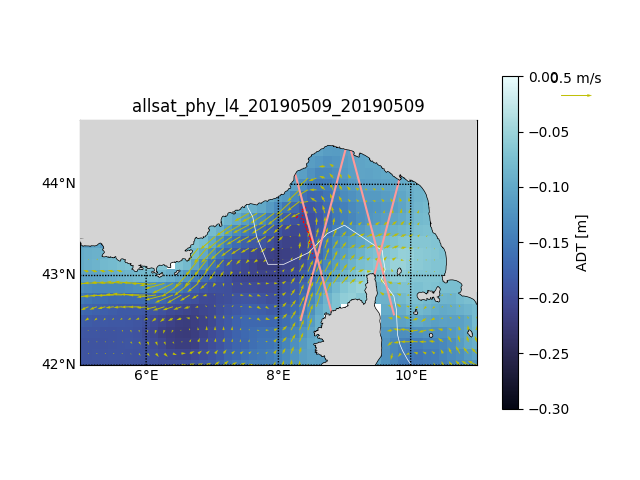
\includegraphics[scale=0.5]{Figures/nrt_med_allsat_phy_l4.png}
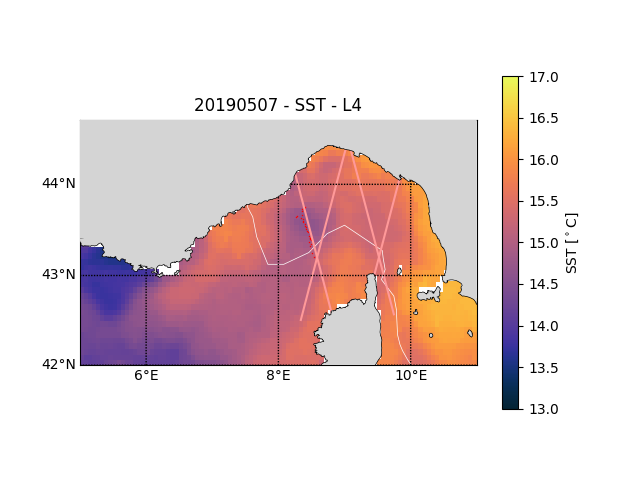
\includegraphics[scale=0.5]{Figures/GOS-L4_GHRSST-SSTfnd-OISST_HR_NRT-MED.png}
\begin{center}
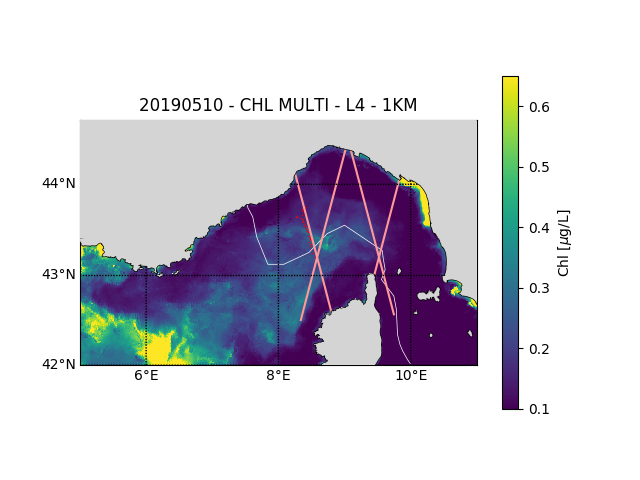
\includegraphics[scale=0.5]{Figures/d-OC_CNR-L4-CHL-INTERP_MULTI_1KM-MED-NRT.png}
\end{center}
\caption{Example of figures: SSH and velocity, SST and CHL concentration}
\end{figure}


%After executing \textit{map\_NRT\_data.sh}, crontab copies images from \texttt{Figures/} into the public\_html file in order to released them on a chosen webpage.\\
%Figures are processed for the entire campaign domain but also "zooms" are realized to focus specificly on the three long duration stations of the campaign. For each map the limits of territorial waters are representated. An example of daily maps is available in Annexe A.    

\newpage
\subsection{Lagrangian analysis}
NetCDF data files are extracted from \texttt{Data/ALTI}, including data for the day.
\begin{itemize}
\item MAIN\_Lagrangian.m: get NetCDF U/V data for the day and previous 30 days to simulate the displacement of particules. \newline

$\rightarrow$ aviso\_load: Chooses different functions to read velocity fields depending on the specified product (dt, nrt, date of products, geographic zone...) \newline

$\rightarrow$ all\_lagrangian\_diags: Launches all the functions to compute the lagrangian diagnostics \newline

\item all\_lagrangian\_figs.py: Plots maps of Lagrangian analysis for the studied zone, using the all\_lagrangian\_diags .mat files from \texttt{Wrk/}, and saves them in .png format.\newline
\end{itemize}
(N.B: $\rightarrow$ = call function)\\ %More details about scripts and contents of \texttt{Lagrangian\_package/} and \texttt{Mfiles/} are available at: \url{file:///home/ENS/apogee/r1003867/Stage_OUTPACE/OUTPACE/doc/index.html}) (à changer avec adresse internet) \newline
\newline
Products of this analysis are generated by the calculation of: \newline
- Lyapunov exponent \newline
- Okubo-Weiss parameter \newline
- Longitude and latitude advection \newline
- Velocities \newline
- Time from bathymetry : represents particules that were on the "plateau".

\begin{figure}[h!]
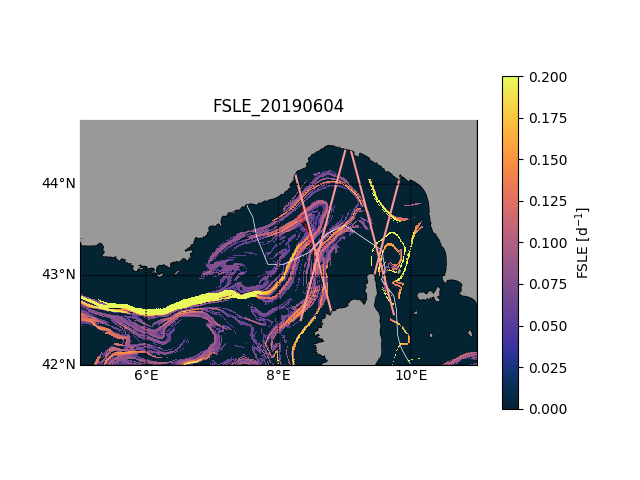
\includegraphics[scale=0.5]{Figures/FSLE.png}
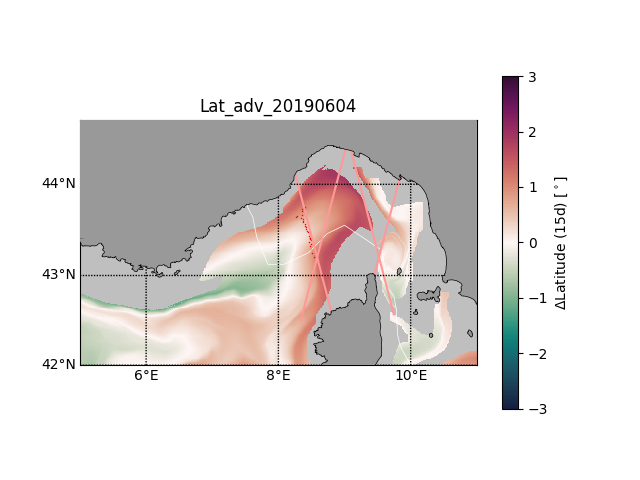
\includegraphics[scale=0.5]{Figures/Lat_adv.png}
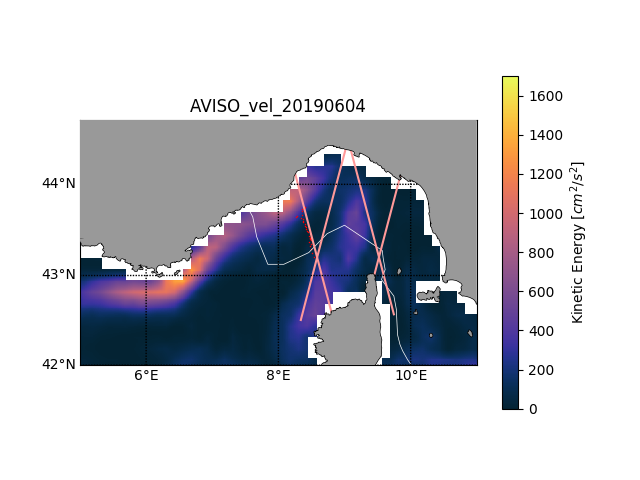
\includegraphics[scale=0.5]{Figures/AVISO_vel.png}
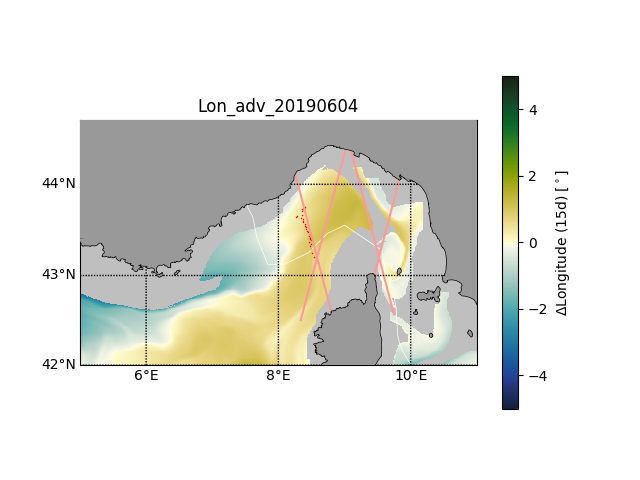
\includegraphics[scale=0.5]{Figures/Lon_adv.png}
%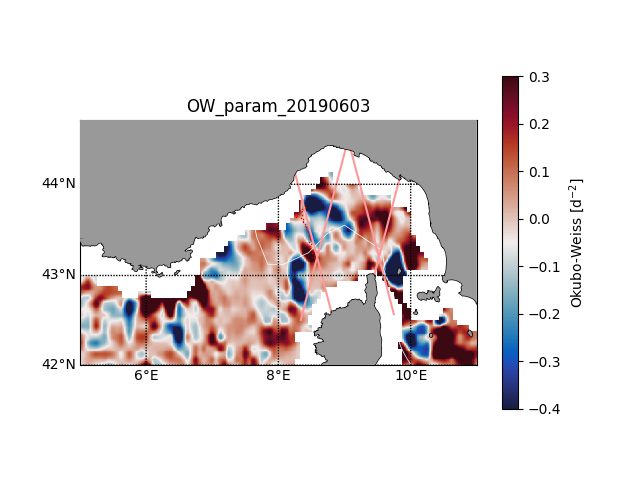
\includegraphics[scale=0.5]{Figures/OW_param.png}
\caption{Example of figures of the LAGRANGIAN analysis: FSLE, latitudinal advection, kinetic energy, longitudinal advection}
%and Okubo-Weiss
\end{figure}

\newpage
\section{Getting Started}
\subsection{Software requirement}
This software requires a Linux OS for bash script to be processed. A recent version of Octave is also needed (tested version was Octave-3.2.3) with hdf4 (need ncdump and ncgen function) and bzip2 intalled and python 2.7.\\
The version of netcdf required is version 3.6.3. Use netcdf version 3.6.3.
For octave, install octave-pkg-dev. Under Linux Debian or Ubuntu apt-get install octave-pkg-deb. Compile the package latma.dev with command makeall in directory Scripts/Lagrangian\_package/lamta.dev/\\
Install Ferret (NOAA) on your computer.\\
Need to have a mail client mutt.\\

\subsection{How to start}
This section sums up all advices you should follow if the scripts do not run well.\\
First of all you only need to adapt the path for your own computer in the first lines of \textit{spasso.sh}. 
Create an account on websites providing products and services of interest
Save your login and password and add them in the first lines of \textit{spasso.sh}. \\

Also make sure that every file exists before running in the bash script. You should follow the same file directory as seen earlier so that you only have to change the "main\_path" in bash script and to be sure to get your files in the right folder. \\
This is the first and only step you have to make to be ready to use this software. When \textit{spasso.sh} is an executable, you can launch it with Linux command: \textbf{./spasso.sh} .\\

At the end of the run, spasso.sh creates a tar file containing all the output figures and remove all the files of the work directory. . The tar file is sent automatically by email.\\
You need to adapt the mailing\_list as you wish in spasso.sh. \\

\subsection{Warning}
Before running \textit{spasso.sh} in crontab make sure that each script gets its arguments from the bash script and not from hard path. \\
\\
Encoded the crontab to run \textit{spasso.sh} when all the release are available on line. Check the arrival times of products for your area, e.g. the \href{https://spasso.mio.osupytheas.fr/FUMSECK/}{FUMSECK} \footnote{https://spasso.mio.osupytheas.fr/FUMSECK/}\textbf{•} cruise. \\
\\
Lagrangian analysis processing needs *.nc.gz files so you have to make sure all NetCDF uv files remain "gzipped" in \texttt{Data/ALTI/} otherwise *.nc files can not be used by the lagrangian scripts.


\newpage
\section{Sampling strategy demo}
To predict boat route, distance and travel time during a station sampling, a new demo was created based on a simple strategy which consists in following the diagonals of a 40km square around the center of the station and then the boat draws a zigzag route inside a smaller square (20km) centered on the center of the station. The MVP\_sampling\_demo.m script is added to the package with the MVP\_sampling\_param.m file which permits the user to change every constant parameter to make the script fit to his needs.\\
This matlab script requires m\_map toolbox to draw the boat route at each time interval defined by the user in the parameter file. A .out file is also processed by the script to record variables that can be useful on board to steer the boat, such as longitude and latitude targeted for each point the boat needs to reach, the direction to follow, the distance traveled (and time) since the navigation started and the time to walk the path.
\begin{figure}[h!] 
\begin{center}
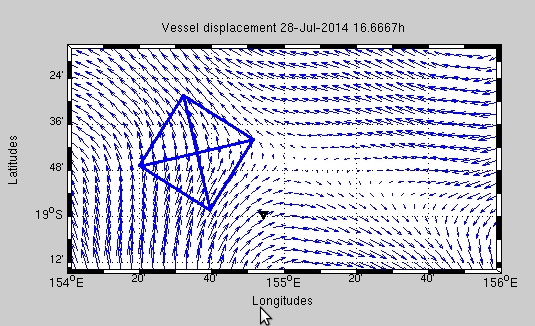
\includegraphics[scale=0.4]{Figures/mvp_sampling_demo.png}
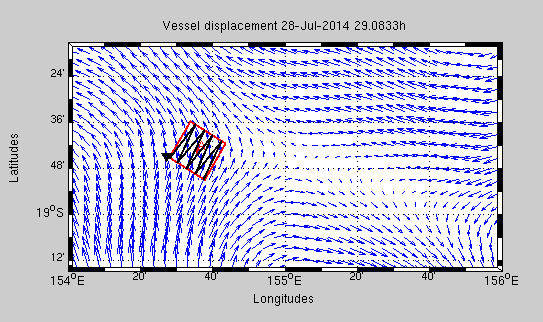
\includegraphics[scale=0.4]{Figures/mvp_sampling_demo2.png}
\caption{Boat route during the MVP sampling strategy. i) Black triangle = boat, ii) Blue square = 40km square, iii) Red square = 20km square.}
\end{center}
\end{figure}

\appendix
\section{Example of daily maps processed for AVISO and MODIS data during the OUTPACE cruise preparation}

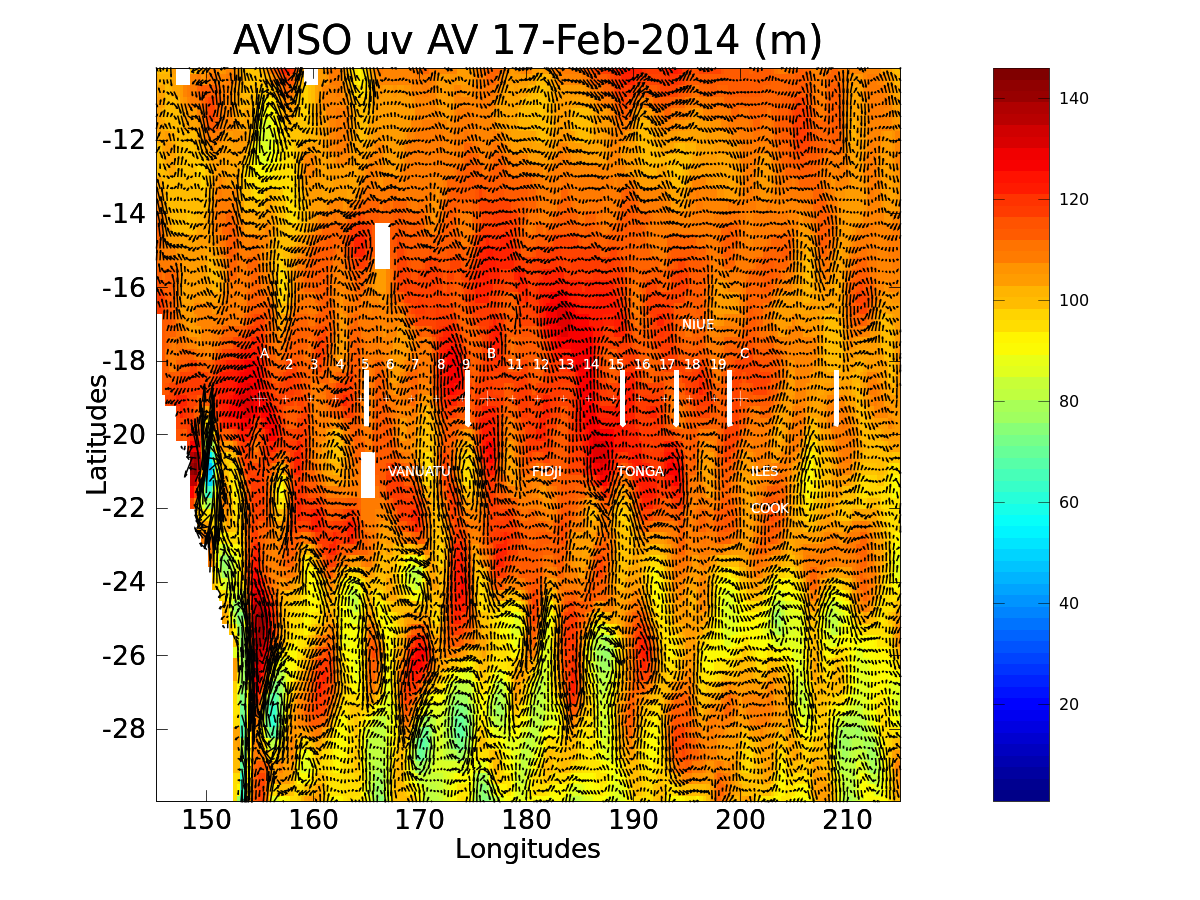
\includegraphics[scale=0.18]{Figures/20140217_AVISO_d0_uv.png}
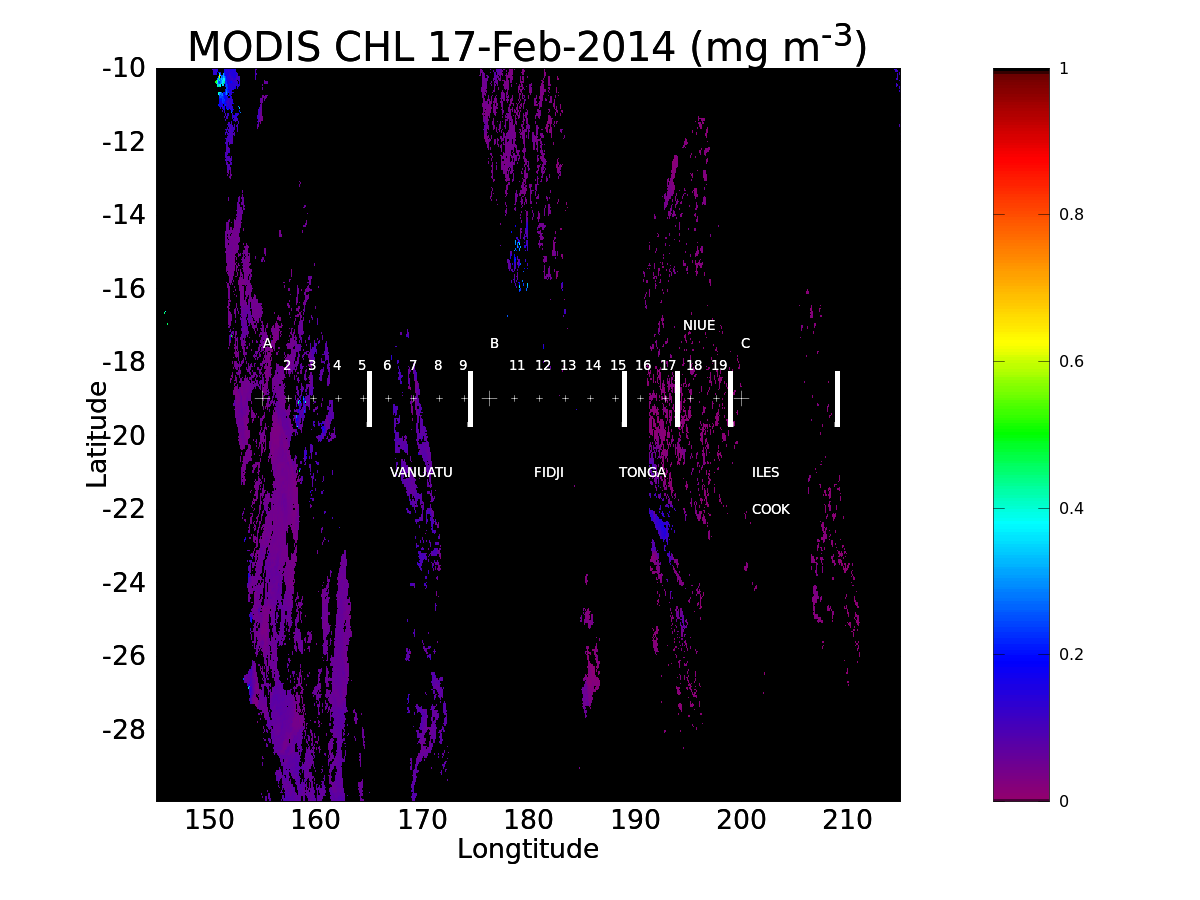
\includegraphics[scale=0.18]{Figures/20140217_MODIS_CHL.png}
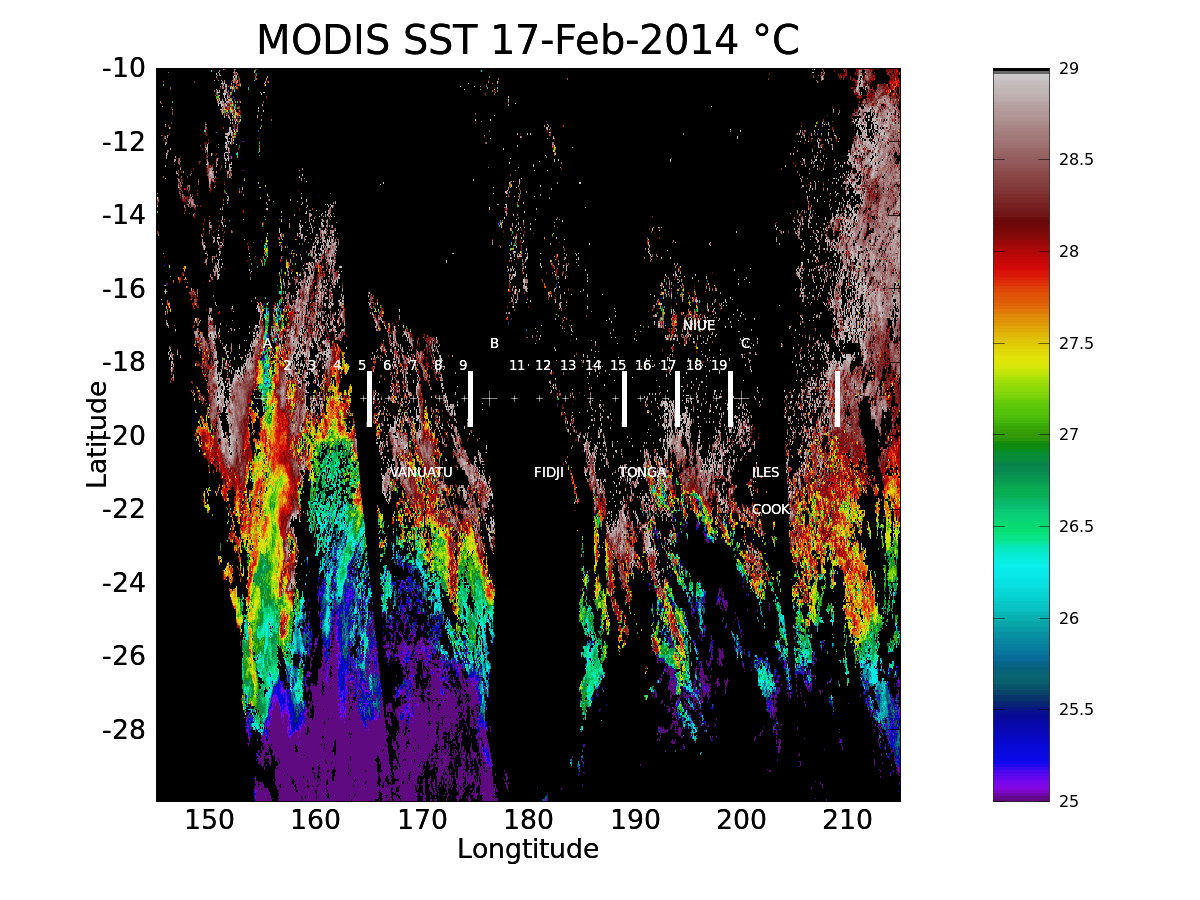
\includegraphics[scale=0.18]{Figures/20140217_MODIS_SST.png}
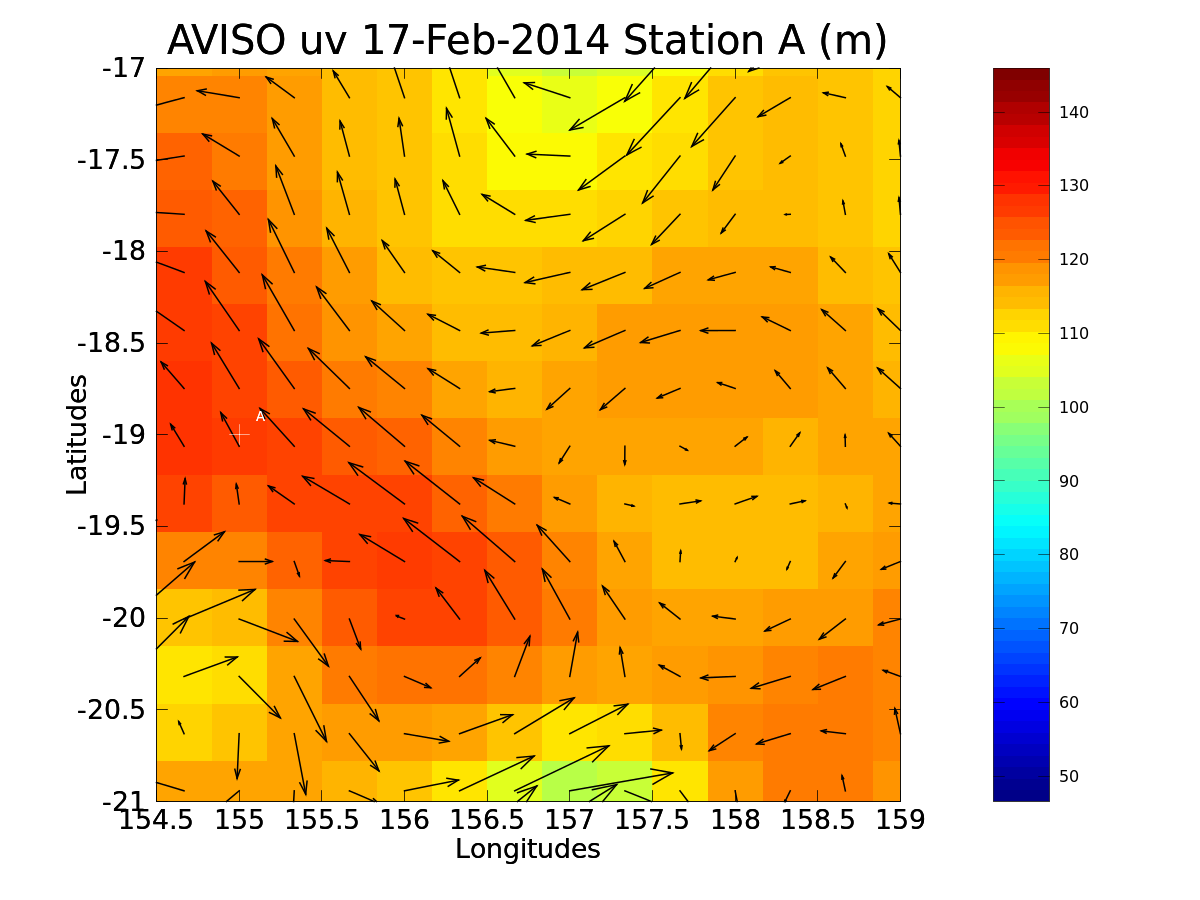
\includegraphics[scale=0.18]{Figures/20140217_AVISO_d0_uv_stationA.png}
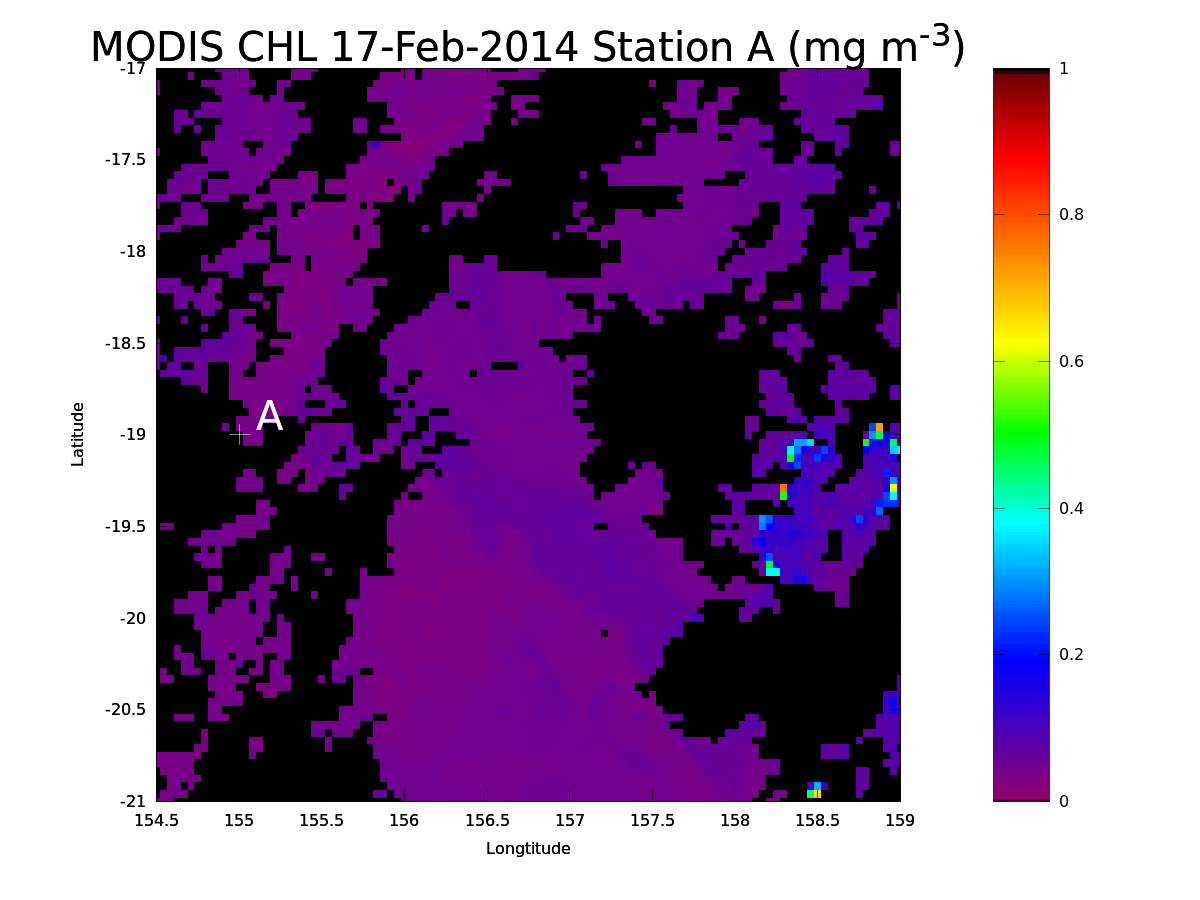
\includegraphics[scale=0.18]{Figures/20140217_MODIS_stationA_CHL.png}
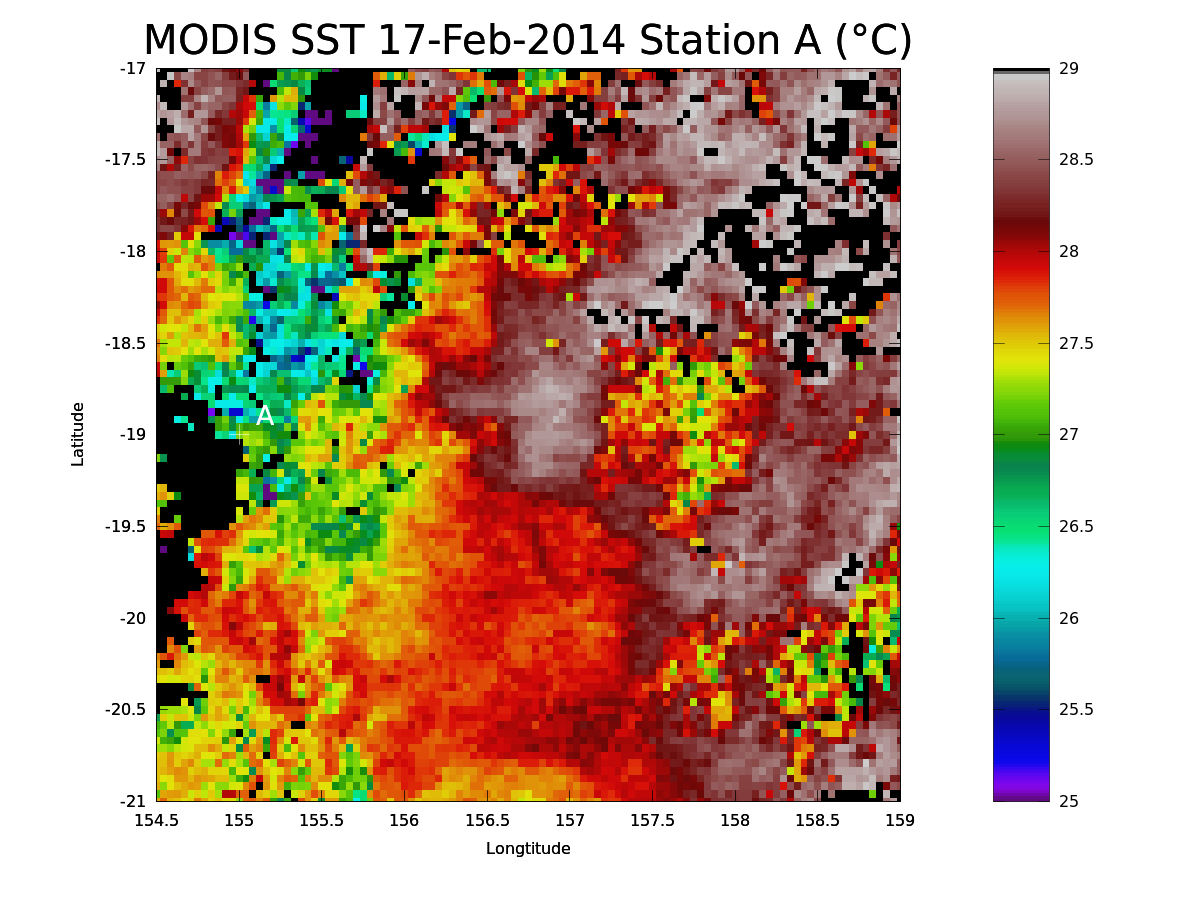
\includegraphics[scale=0.18]{Figures/20140217_MODIS_stationA_SST.png}
Maps processed by \textit{map\_NRT\_data.sh} for the entire domain and the first long duration station (A). Same maps are available for stations B and C.


\end{document}
